\subsubsection{Rotator head}
\subsubsection*{Concept Overview}
The basic concept of the rotation mechanism relies on an assortment of three bevel gears set up in a T-configuration. The central shaft would be mounted vertically to the main mount and the other collinear shafts each attached to an individual JGY 370 12 V DC motor. The action of these motors against the gear assembly would allow for rotation in both the azimuth and elevation directions. This is achieved through attaching an inverted U-shaped aluminum bracket that forms the main fixture structure of the whole rotator. The sides of the bracket are each attached to one of the driven shafts and their relevant motors, while the top face serves as the mounting location of the antenna and printed circuit boards including the Raspberry Pie 4.\\
When the opposing motors rotate in the same direction i.e. both clockwise, the gears are able to transform this into movement in the azimuth direction. This is due to the reaction against the central fixed gear.\\
However, when ordered to rotate in opposing directions this is translated into gears rotating in the same direction against the central gear. This of course will not be physically possible and hence the gear point is fixed, and the rotation motion is transferred to the motors themselves around the axis and by that consequently moving the bracket up or down, changing the elevation sense of the antenna.

\begin{figure}[H]
	\centering
	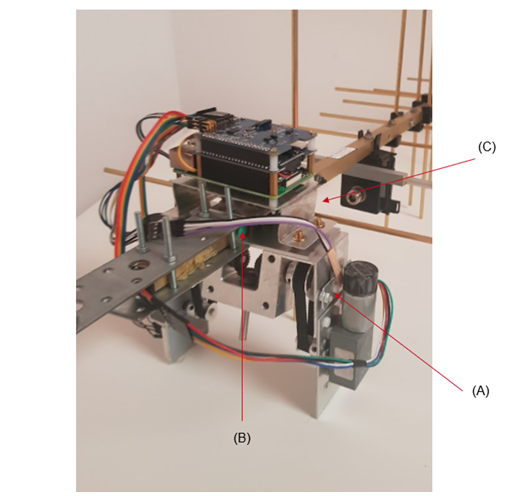
\includegraphics[width=0.8\textwidth]{../art/Pic1Head.png}
	\caption{Rotator Head without shielding.}
\end{figure}

\subsubsection*{Design} 
The initial conditions to be met were the first driving parameters for the design. Namely, the required torque was first investigated. Assuming that this portable rotator would not be tested in storms, the highest of the average of wind speeds in Germany was considered, that being during January, and then rounded to get 19.5 km/h. Since we imagined using a cross Yagi antenna for this application, we took into account one face of the boom and calculated the area to be 0.15 m\^2, the directors being cylindrical and of small diameter were also estimated and found to be of negligible effect if exposed to wind drag. This put together along with the reflector and other parts did not amount to much in relation to torque requirements. The torque required was calculated to be less than 0.25 N however we decided to use this value for safety, and to allow more flexibility for use with other types or shapes of antennas. Separately the average torque of one motor was found to be around 1.3 N/m. While this was sufficient and tested on the first prototype to be adequate for controlling the rotator with a dummy weight, we later decided to double this potential by two, and this was achieved by utilizing a belt and pulley system with a ratio of 2:1.\\
The belts and pulleys in concern are those of GT2 pulleys, and 9mm timing belts. The same class of belts and pulleys used in most commercial 3D printers. This design decision seemed logical for two reasons, one being the need of precise movement and transmission without slippage as is the case for 3D printers, and the other being the affordability and availability characteristics of said parts. A permanent relative position and a constant speed ratio are easy to expect using this product while also being able to handle heavy loads. [1]\\
Constrained by the purchased belt length\footnote{Due to logistics the favored belt length could not be available within time and the design was iterated to fit a new belt.} and the available GT2 pulleys we could finally define the distance between the centers of the horizontal gear and motor shafts. This parameter would also aid in defining the length of the side member of the main bracket to allow for this assembly while taking into account mounting locations of other components of the system. \\
This distance mentioned earlier would be the distance required between the pulleys to fit the belt effectively and ensure efficient functionality. We determined this distance by first investigating the outer diameters of each pulley and then plugging it along with the belt length into this equation:\\
\begin{center}
    $\frac{b+ \sqrt{b^2-32(D-d)^2} }{16}=C$
\end{center}
Where $b=4L-6.28(D+d)$, D: Diameter of large pulley, d: Diameter of small pulley, and L = Length of the belt.\\
Another approach was by using the number of teeth of each pulley after determining the tooth style or pitch which is 2mm for our case.\\
\\
The other main distance to be defined for the bracket was the length. This describes the distance between the inner faces of the opposing sides. Those sides are assigned to support both horizontal axis of the gears. Considering many variables, such as dimensional, geometric, and support characteristics of available pillow block flange bearings, gear shaft length, sheet material thickness, and pulley sizes, the final length was defined at 12.3 cm. However, later this value was changed to 13.5 cm due to changes carried out to meet shortcomings in logistics again. This was still achievable by changing multiple aspects of the design to still be able and accommodate the bearings and shafts as required. 
\\
The final two and not very challenging dimensions to define were the width of the bracket and the mounting location of the driven shafts from the upper face of the bracket.
\\
Further into the build, two 6 mm tubes were threaded to fit into the motor shafts as extensions so we can manage to align the pulleys properly. Bushings were added at the end of each horizontal gear shaft right where they interface with the side bearings. These bushings were also drilled as required to allow the bearing's fasteners to go through them and hold onto the shafts. This is due to having the bearings at 8 mm diameter while the shafts are of a 6 mm diameter. These same bushing also serve to protect the magnets glued at the end of the shafts from getting too close to the metallic balls of the bearing\footnote{This is not a concern anymore, however in a previous method of attachment, for a worst case scenario if the magnet miss-aligns for any reason it would still rotate with the shaft as it doesn't get close enough for it to be pulled to one side alone.}. The latter mentioned magnets are positioned as such to allow reading the position of the shaft by two encoders, each mounted on one side of the bracket. Special mounting plates (A) were designed, cut, and drilled to situate those encoders at the right proximity from the magnets. According to our tests a distance beyond 5 mm was sufficient to lose a proper reading and hence we ultimately managed to install them within a clearance of 1 mm for best reading. Spacers were added between the motors and bracket faces to distance the motor ends from the encoders, while both isolating a chance of interference due to the rotating magnet of the motor's encoders and also allowing easy installation and removal of the encoders in case of inspection or issue without having to uninstall the motors and other components of the assembly first.

\subsubsection*{Material Selection}
The antenna at hand weighs no more than 0.5 kg. When balanced in its mounting location on the bracket, the only load of concern is that applying directly downwards on the bridge. A secondary concern would be the torsional load on the same plate when the rotator moves at its lateral axis. Several design solutions were planned, however using the final procurement, it was found that this issue is easily treated by using an aluminum plate thickness of 3 mm. It must be noted that this was not possible in the initial design because a thickness more than 2 mm for the sides would result in other considerations because we are constrained by certain dimensions of the bearing flanges which would lead to disruption of other parameters as well. However, using the modular approach, we were able to simply use an aluminum plate of a larger thickness for the top section.\\
\\
A FEM analysis shows how the current design handles the load of the antenna.\\
\\
(Include simulation here.) Figure.

\subsubsection*{Antenna Strainer}
The design for the antenna mount varied. Two similar concepts were finally tracked, one would be using a bent aluminum sheet, and another is 3D printed.\\
\\
Note: The metal sheet work required a wait time of two weeks in the workshop due to a busy schedule, and the 3D printed part was never delivered as technical problems with the printer were reported during the job.
\begin{figure}[H]
\centering
\begin{subfigure}{.5\textwidth}
  \centering
  \includegraphics[width=.85\linewidth]{../art/Strain1.png}
  \caption{Machined part.}
  \label{fig:sub1}
\end{subfigure}%
\begin{subfigure}{.5\textwidth}
  \centering
  \includegraphics[width=.85\linewidth]{../art/Strain2.png}
  \caption{3D printed part.}
  \label{fig:sub2}
\end{subfigure}
\caption{This figure shows two of the final antenna holders.}
\label{fig:test}
\end{figure}
On the final presentation the antenna was fixed using a sandwich of aluminum plates, constrained by 3 bolts on each side, and wrapped in a rubber material (B) as an interface between the antenna boom and the bolts and plates to increase traction considerably and avoid any chance of slippage during operation (Figure 2).

\subsubsection*{PCB Mounting}
A custom-made bridge (C) was drawn and fabricated to mount the PCB sandwich (Figure 2).
